%%%%%%%%%%%%%%%%%%%%%%%%%%%%%%%%%%%%%%%%%%
\section{Esperimenti}
\frame{\frametitle{Ciclo di lavoro}
\centering
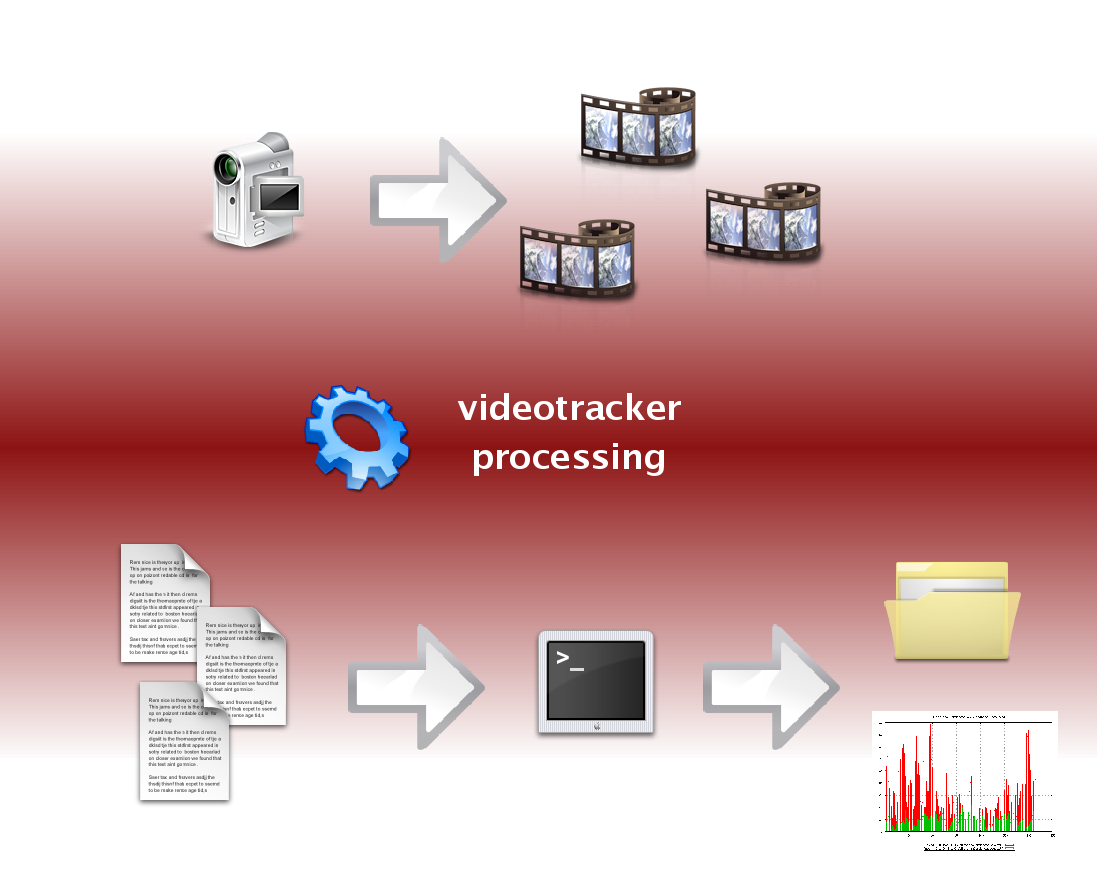
\includegraphics[scale=0.35]{img/Presentazione.png}

}

%%%%%%%%%%%%%%%%%%%%%%%%%%%%%%%%%%%%%%%%%%
\frame{\frametitle{Parametri e output}
\begin{small}\alert{\textbf{Esperimenti}}: variazione di tre parametri nei tre video selezionati \end{small}
\begin{footnotesize}\begin{description}
\item [Intervallo Frames] Numero di frames tra due applicazioni consecutive del Tracking
\item [Q - Area Kalman] Autovalori di Q, risulta l'area di confidenza del filtro di Kalman
\item [Samples ConDensation] Numero di samples sui quali si basa l'esecuzione del ConDensation
 \end{description}\end{footnotesize}\pause
\begin{block}{}
\begin{footnotesize}Il software produce sei files di output:\end{footnotesize}
\begin{scriptsize}\begin{description}
\item [\textit{coordinateReali.txt}] Coordinate reali dell'oggetto da tracciare
\item [\textit{coordinateKalman.txt}] Coordinate previste da Kalman
\item [\textit{coordinateCondensation.txt}] Coordinate previste dal ConDensation
\item [\textit{distanzaKalman.txt}] \alert{$\delta_k$} Distanza tra le coordinate reali e la previsione di Kalman
\item [\textit{distanzaCondensation.txt}]\alert{$\delta_c$} Distanza tra coord reali e previsione ConDensation
\item [\textit{Risultati.txt~~~~~~~~~~~}]  distanza media, $\overline{\delta}_k, \overline{\delta}_c$, varianza media ConDensation ($\overline{\sigma}_x, \overline{\sigma}_y$).
 \end{description}\end{scriptsize}
\end{block}
}

%%%%%%%%%%%%%%%%%%%%%%%%%%%%%%%%%%%%%%%%%%
\frame{\frametitle{GNUPlot - plot.png}
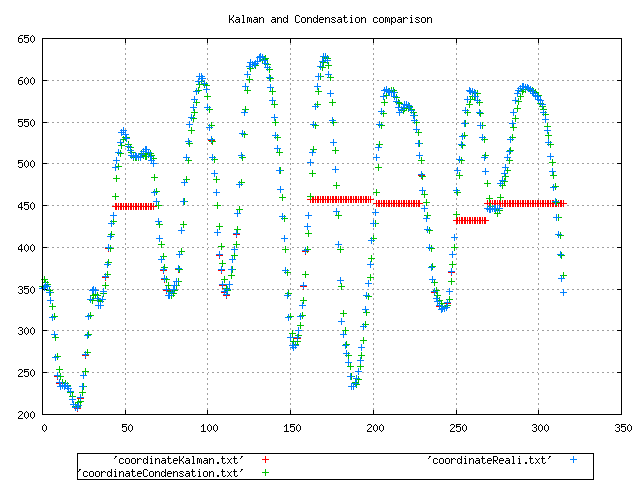
\includegraphics[scale=0.45]{../esperimenti/movie12/mod_3-Q_1000-S_1000/plot.png}

}

%%%%%%%%%%%%%%%%%%%%%%%%%%%%%%%%%%%%%%%%%%
\frame{\frametitle{GNUPlot - distances.png}
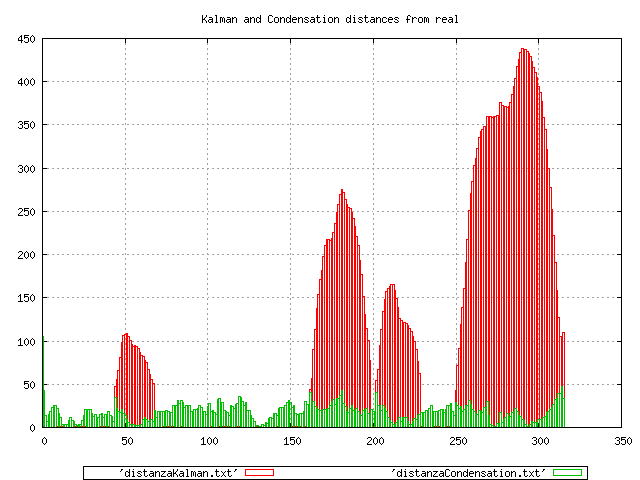
\includegraphics[scale=0.45]{../esperimenti/movie12/mod_3-Q_1000-S_1000/plot-distances.png}
}

%%%%%%%%%%%%%%%%%%%%%%%%%%%%%%%%%%%%%%%%%%
\subsection{Video}

\frame{\frametitle{Primo video - movie12.mjpeg}
\begin{columns}
\column{.65\textwidth}
\begin{small}\begin{itemize}
 \item occlusione, moto circolare e costante
\item 640x480, 25$fps$, 50.4$s$
\end{itemize}\end{small}

\column{.35\textwidth}\centering
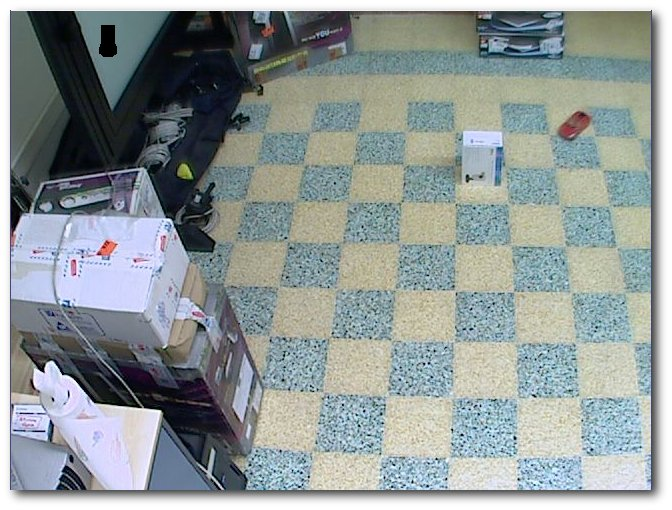
\includegraphics[scale=0.15]{../relazione/figure/movie12.jpg}
\end{columns}
\begin{columns}

\column{.20\textwidth}
\begin{scriptsize}
\begin{itemize}
\item [M]3
\item [Q]1000
\item [S]1000
\end{itemize}
\end{scriptsize}
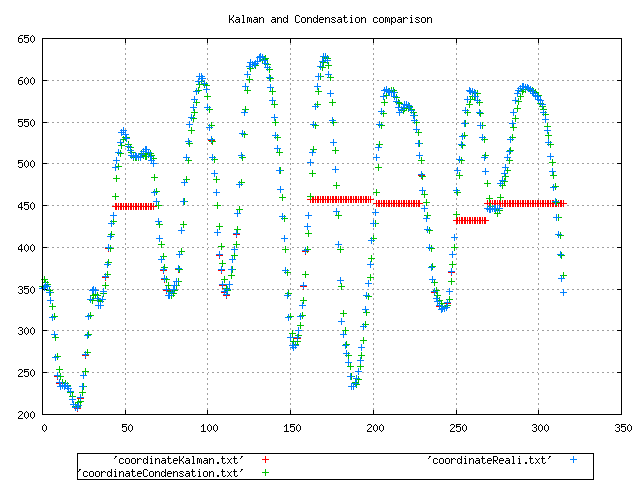
\includegraphics[scale=0.1]{../esperimenti/movie12/mod_3-Q_1000-S_1000/plot.png}\\
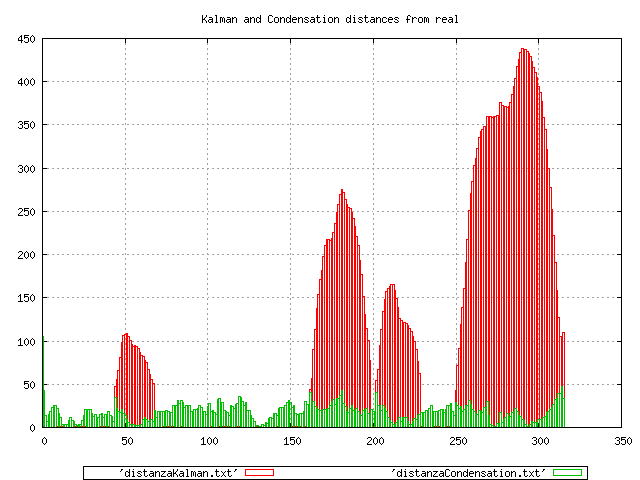
\includegraphics[scale=0.1]{../esperimenti/movie12/mod_3-Q_1000-S_1000/plot-distances.png}

\column{.20\textwidth}
\begin{scriptsize}
\begin{itemize}
\item [M]3
\item [Q]2000
\item [S]1000
\end{itemize}
\end{scriptsize}
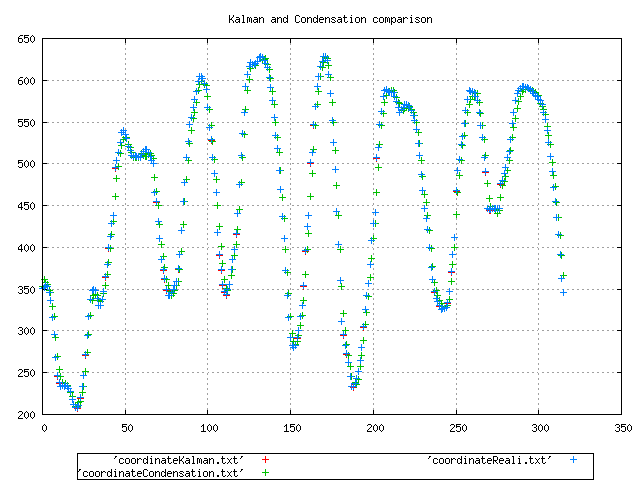
\includegraphics[scale=0.1]{../esperimenti/movie12/mod_3-Q_2000-S_1000/plot.png}\\
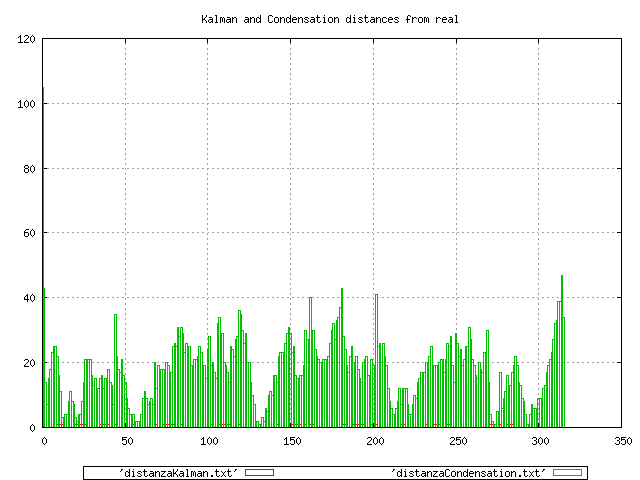
\includegraphics[scale=0.1]{../esperimenti/movie12/mod_3-Q_2000-S_1000/plot-distances.png}

\column{.20\textwidth}
\begin{scriptsize}
\begin{itemize}
\item [M]3
\item [Q]1000
\item [S]5000
\end{itemize}
\end{scriptsize}
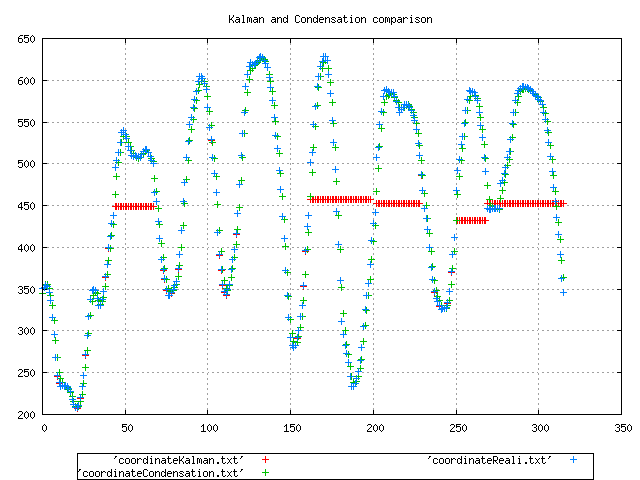
\includegraphics[scale=0.1]{../esperimenti/movie12/mod_3-Q_1000-S_5000/plot.png}\\
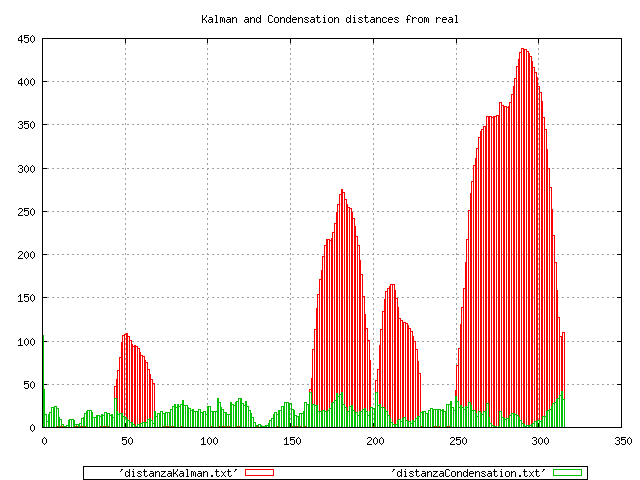
\includegraphics[scale=0.1]{../esperimenti/movie12/mod_3-Q_1000-S_5000/plot-distances.png}

\column{.20\textwidth}
\begin{scriptsize}
\begin{itemize}
\item [M]3
\item [Q]1000
\item [S]100
\end{itemize}
\end{scriptsize}
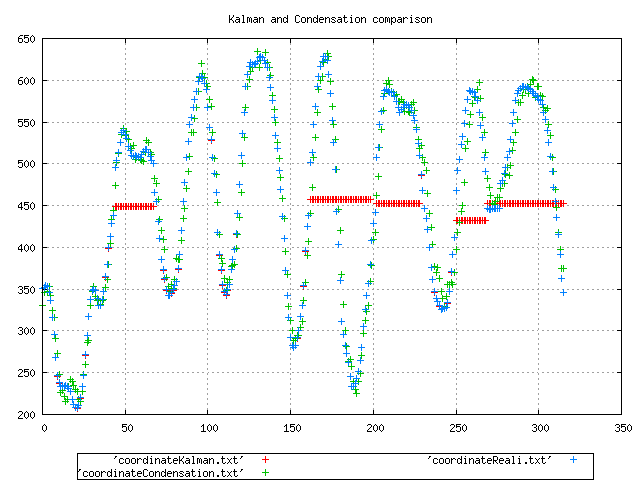
\includegraphics[scale=0.1]{../esperimenti/movie12/mod_3-Q_1000-S_100/plot.png}\\
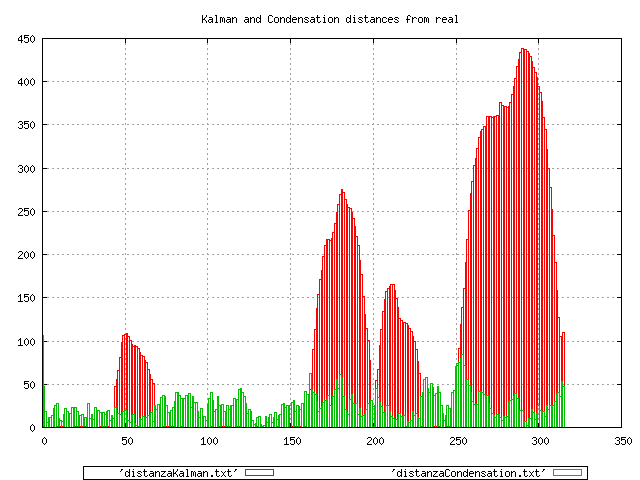
\includegraphics[scale=0.1]{../esperimenti/movie12/mod_3-Q_1000-S_100/plot-distances.png}
\end{columns}

}
%%%%%%%%%%%%%%%%%%%%%%%%%%%%%%%%%%%%%%%%%%
\frame{\frametitle{Secondo video - tappetonozoom.avi}
\begin{columns}
\column{.65\textwidth}
\begin{small}\begin{itemize}
 \item moto vario, repentine accelerazioni, oggetto entra ed esce dalla scena
\item 320x240, 10$fps$, 59$s$
\end{itemize}\end{small}

\column{.35\textwidth}\centering
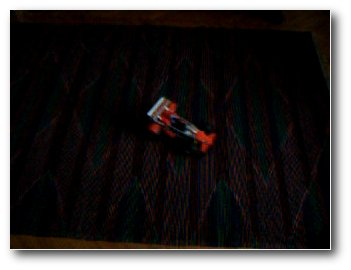
\includegraphics[scale=0.25]{../relazione/figure/tappeto_nozoom.jpg}
\end{columns}
\begin{columns}

\column{.20\textwidth}
\begin{scriptsize}
\begin{itemize}
\item [M]3
\item [Q]1000
\item [S]1000
\end{itemize}
\end{scriptsize}
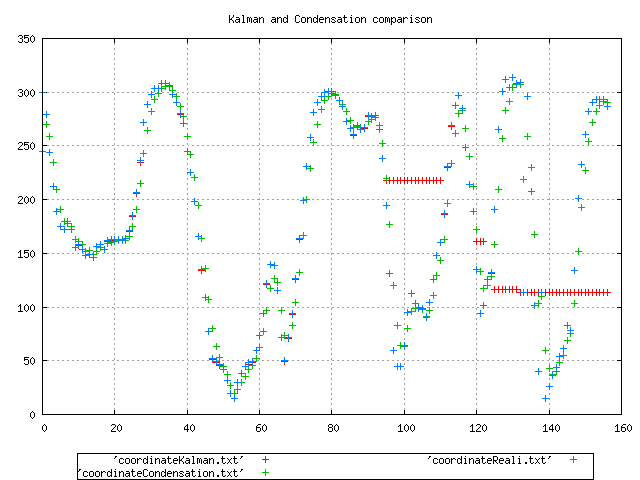
\includegraphics[scale=0.1]{../esperimenti/tappeto_nozoom/mod_3-Q_1000-S_1000/plot.png}\\
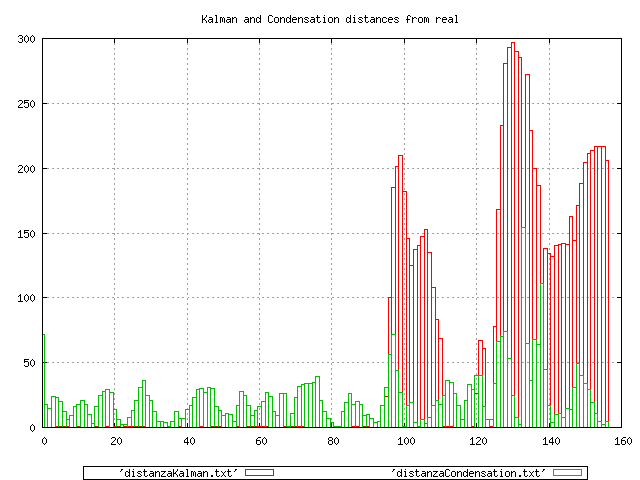
\includegraphics[scale=0.1]{../esperimenti/tappeto_nozoom/mod_3-Q_1000-S_1000/plot-distances.png}

\column{.20\textwidth}
\begin{scriptsize}
\begin{itemize}
\item [M]5
\item [Q]1000
\item [S]1000
\end{itemize}
\end{scriptsize}
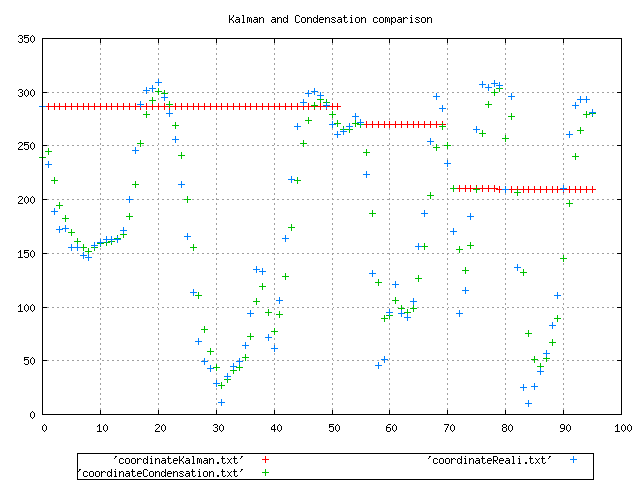
\includegraphics[scale=0.1]{../esperimenti/tappeto_nozoom/mod_5-Q_1000-S_1000/plot.png}\\
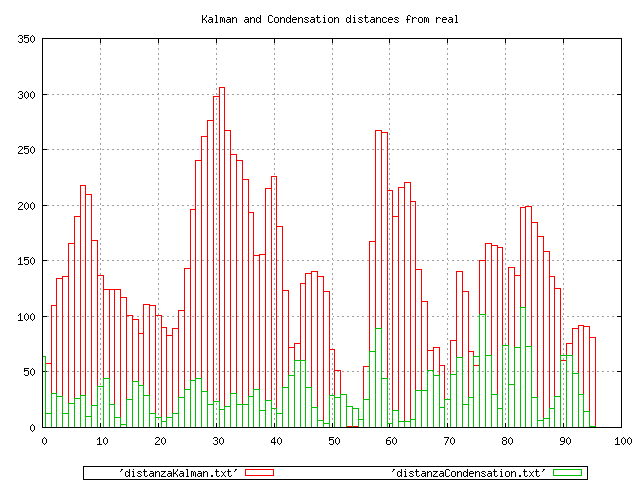
\includegraphics[scale=0.1]{../esperimenti/tappeto_nozoom/mod_5-Q_1000-S_1000/plot-distances.png}


\column{.20\textwidth}
\begin{scriptsize}
\begin{itemize}
\item [M]2
\item [Q]1000
\item [S]1000
\end{itemize}
\end{scriptsize}
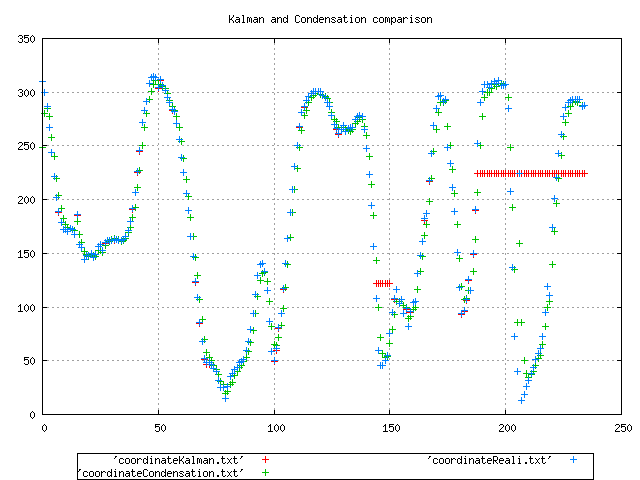
\includegraphics[scale=0.1]{../esperimenti/tappeto_nozoom/mod_2-Q_1000-S_1000/plot.png}\\
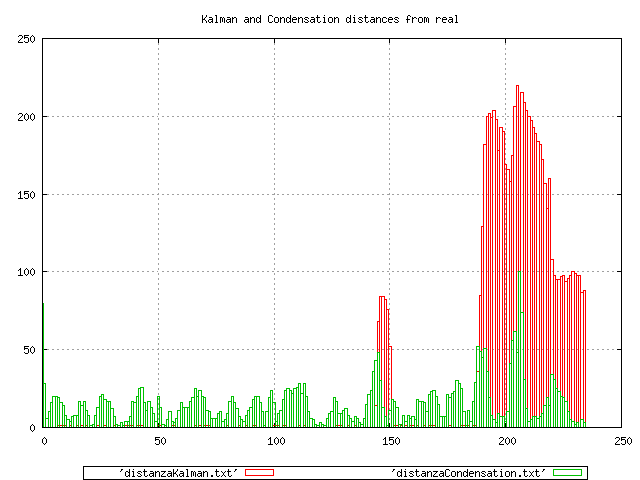
\includegraphics[scale=0.1]{../esperimenti/tappeto_nozoom/mod_2-Q_1000-S_1000/plot-distances.png}


\column{.20\textwidth}
\begin{scriptsize}
\begin{itemize}
\item [M]1
\item [Q]2000
\item [S]1000
\end{itemize}
\end{scriptsize}
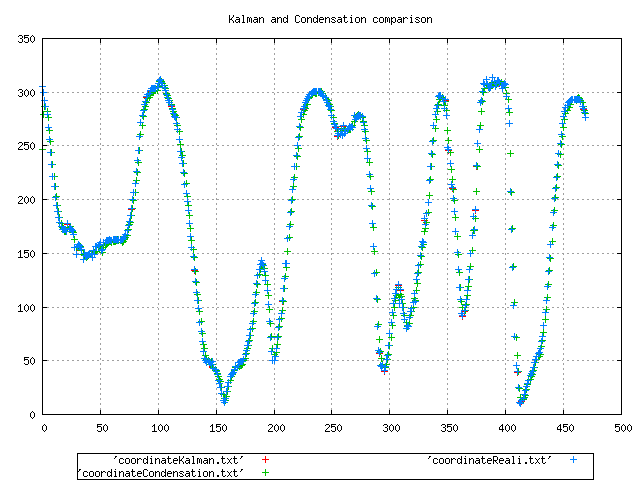
\includegraphics[scale=0.1]{../esperimenti/tappeto_nozoom/mod_1-Q_2000-S_1000/plot.png}\\
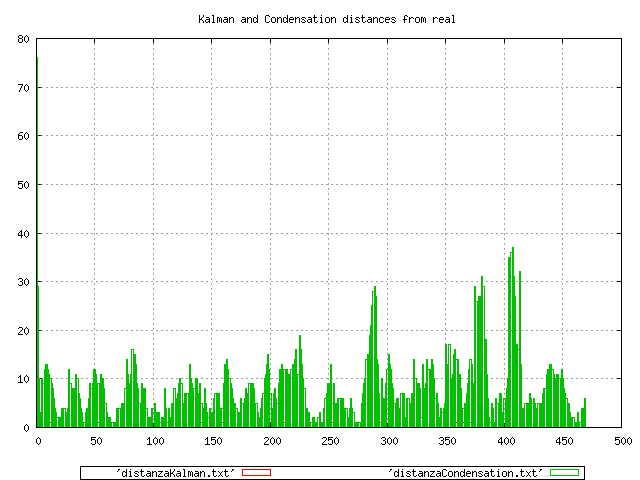
\includegraphics[scale=0.1]{../esperimenti/tappeto_nozoom/mod_1-Q_2000-S_1000/plot-distances.png}
\end{columns}

}
%%%%%%%%%%%%%%%%%%%%%%%%%%%%%%%%%%%%%%%%%%
\frame{\frametitle{Terzo video - singlecar.avi}
\begin{columns}
\column{.65\textwidth}
\begin{small}\begin{itemize}
 \item moto costante, oggetto entra ed esce dalla scena
\item 648x484, 30$fps$, 33$s$
\end{itemize}\end{small}

\column{.35\textwidth}\centering
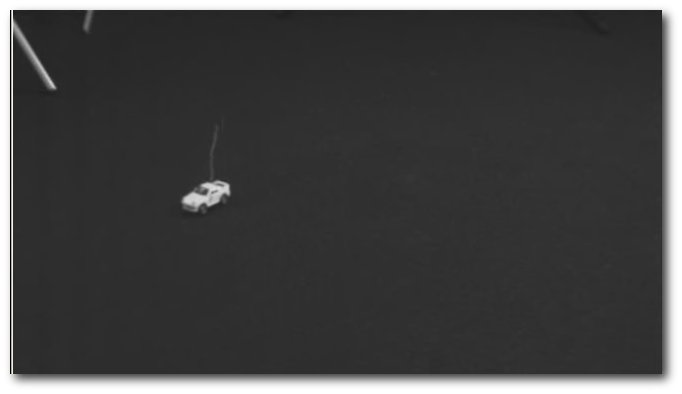
\includegraphics[scale=0.15]{../relazione/figure/singlecar.jpg}
\end{columns}
\begin{columns}

\column{.20\textwidth}
\begin{scriptsize}
\begin{itemize}
\item [M]3
\item [Q]1000
\item [S]1000
\end{itemize}
\end{scriptsize}
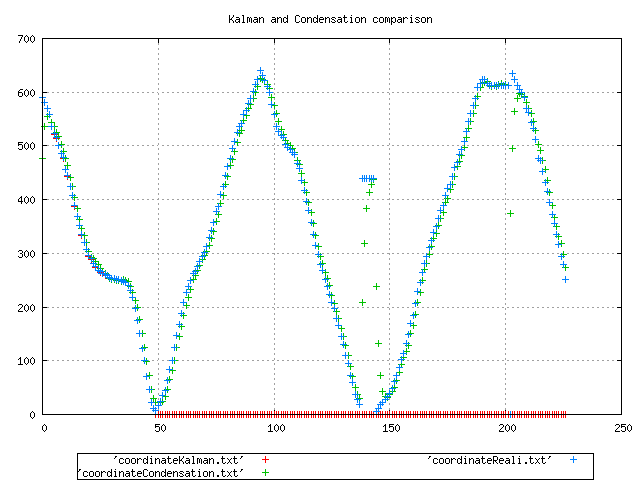
\includegraphics[scale=0.1]{../esperimenti/single_car/mod_3-Q_1000-S_1000/plot.png}\\
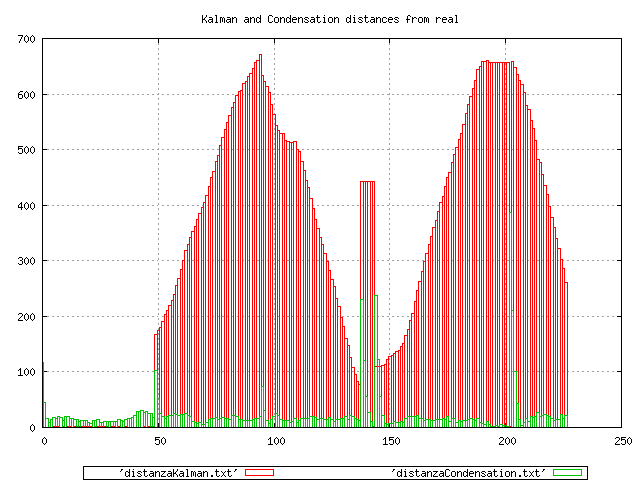
\includegraphics[scale=0.1]{../esperimenti/single_car/mod_3-Q_1000-S_1000/plot-distances.png}

\column{.20\textwidth}
\begin{scriptsize}
\begin{itemize}
\item [M]10
\item [Q]5000
\item [S]1000
\end{itemize}
\end{scriptsize}
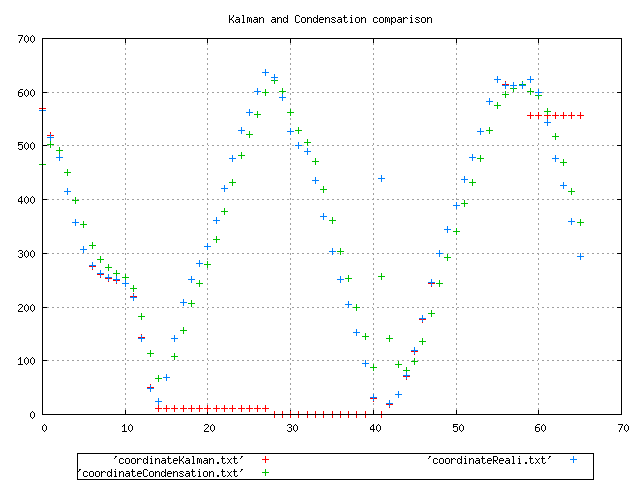
\includegraphics[scale=0.1]{../esperimenti/single_car/mod_10-Q_5000-S_1000/plot.png}\\
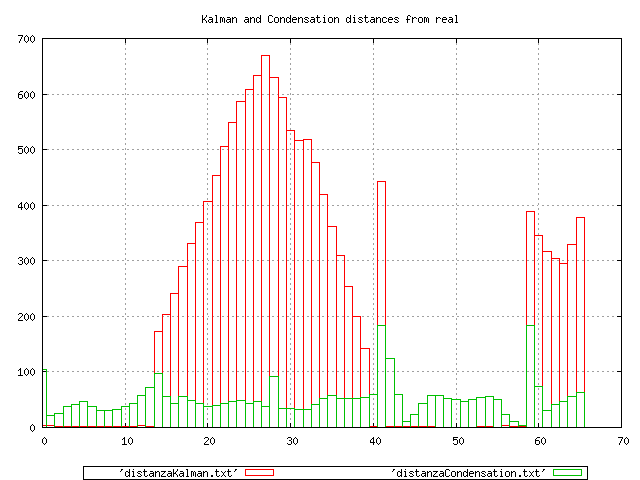
\includegraphics[scale=0.1]{../esperimenti/single_car/mod_10-Q_5000-S_1000/plot-distances.png}

\column{.20\textwidth}
\begin{scriptsize}
\begin{itemize}
\item [M]6
\item [Q]0.1
\item [S]1000
\end{itemize}
\end{scriptsize}
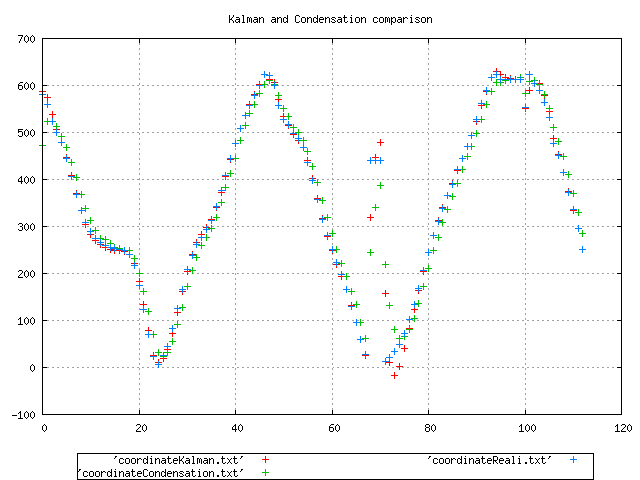
\includegraphics[scale=0.1]{../esperimenti/single_car/mod_6-Q_0.1-S_1000/plot.png}\\
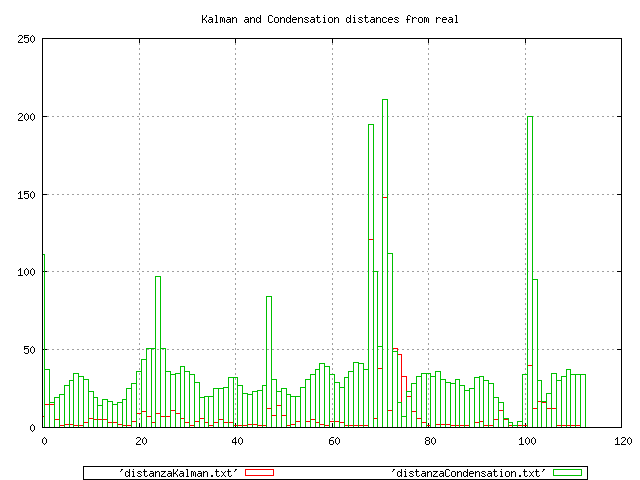
\includegraphics[scale=0.1]{../esperimenti/single_car/mod_6-Q_0.1-S_1000/plot-distances.png}

\column{.20\textwidth}
\begin{scriptsize}
\begin{itemize}
\item [M]1
\item [Q]0.0001
\item [S]1000
\end{itemize}
\end{scriptsize}
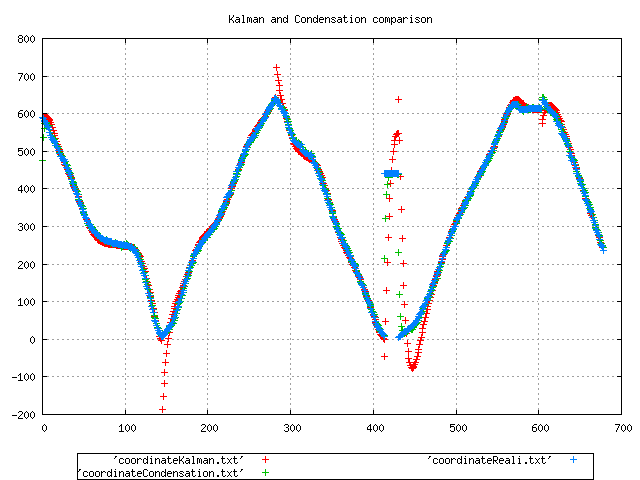
\includegraphics[scale=0.1]{../esperimenti/single_car/mod_1-Q_0.0001-S_1000/plot.png}\\
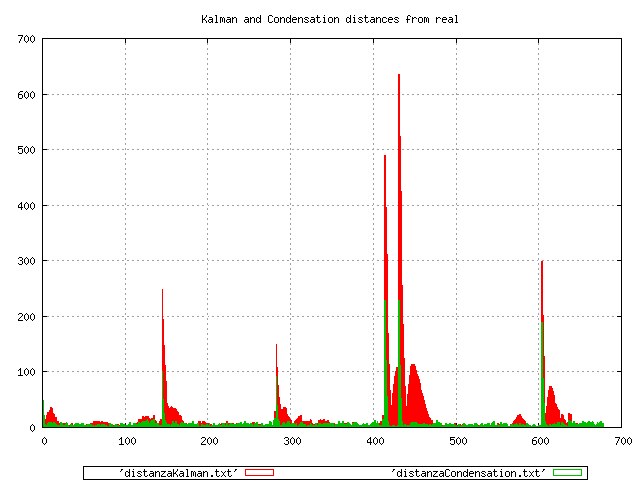
\includegraphics[scale=0.1]{../esperimenti/single_car/mod_1-Q_0.0001-S_1000/plot-distances.png}
\end{columns}
}
%%%%%%%%%%%%%%%%%%%%%%%%%%%%%%%%%%%%%%%%%%
\subsection{Risultati}
\frame{\frametitle{Esperimento 1}

}

%%%%%%%%%%%%%%%%%%%%%%%%%%%%%%%%%%%%%%%%%%
\frame{\frametitle{Esperimento 2}

}

%%%%%%%%%%%%%%%%%%%%%%%%%%%%%%%%%%%%%%%%%%
\frame{\frametitle{Esperimento 3}

}
